\section{Measurements}
\label{sec:measurements}
In order to quantify the performance of the Parallella board and our LSH based KNN search, we measure several parameters such as:
\begin{itemize}
\item Computation time of n\"{a}ive KNN search
\item Computation time of LSH based KNN search
\item Power consumption of Parallella board
\end{itemize}
\subsection{N\"{a}ive KNN Search computation time}
\label{subsec:nknn_comptime}
\begin{figure}
\centering
\begin{subfigure}[b]{0.3\textwidth}
	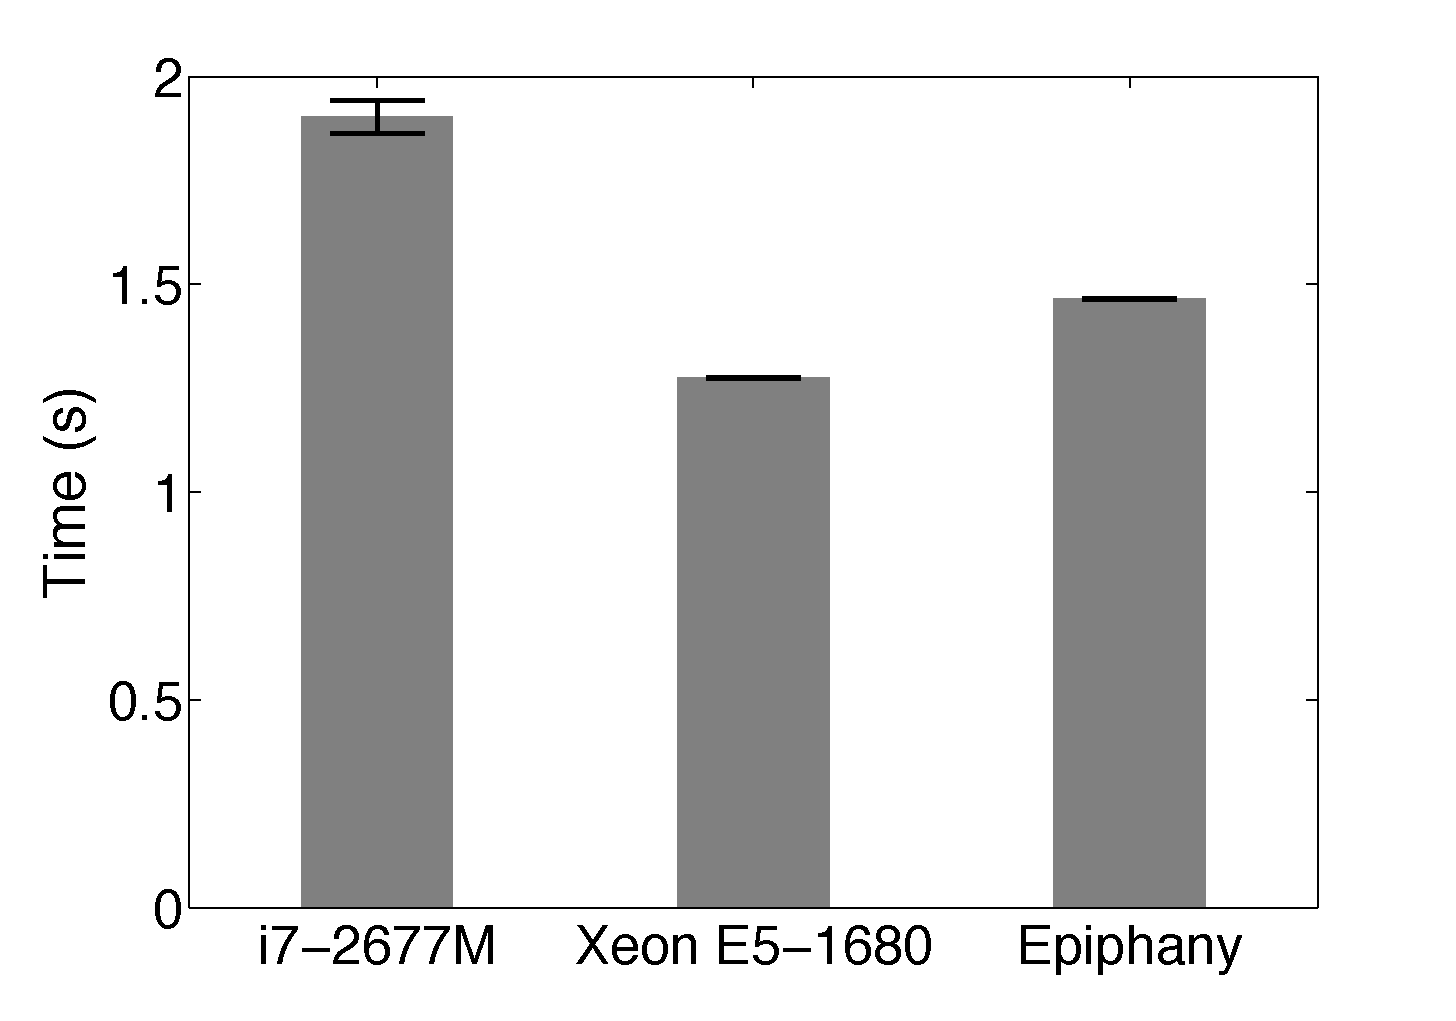
\includegraphics[width=\textwidth]{gt_256.pdf}
	\caption{256 records}
	\label{fig:k256_comptime}
\end{subfigure}
~
\begin{subfigure}[b]{0.3\textwidth}
	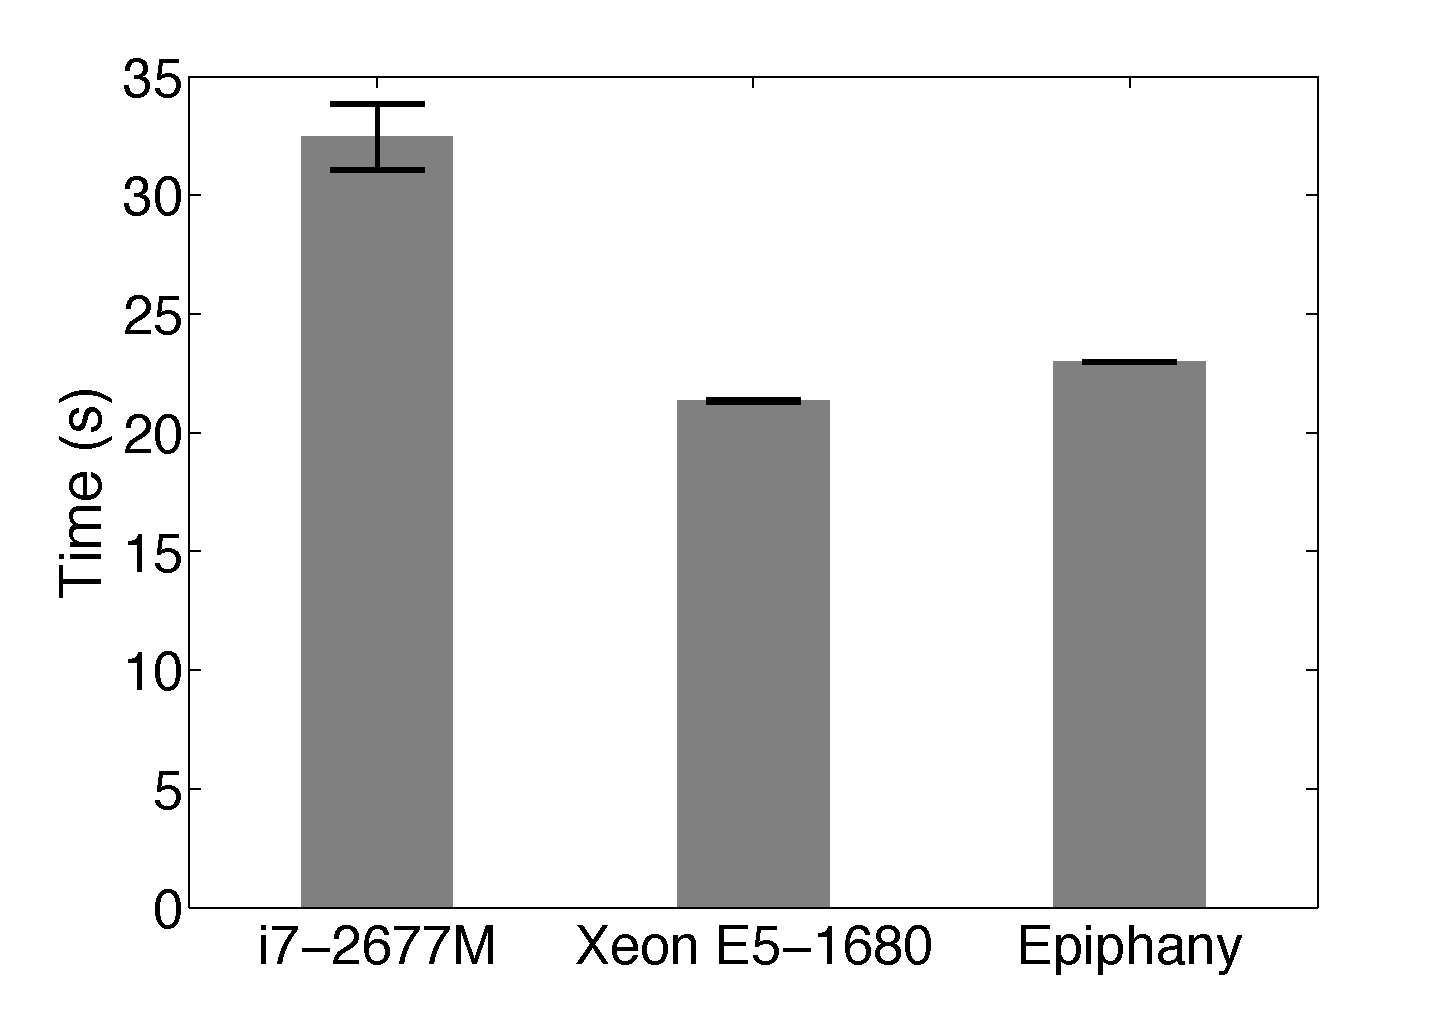
\includegraphics[width=\textwidth]{gt_1000.pdf}
	\caption{1000 records}
	\label{fig:k1000_comptime}
\end{subfigure}
\begin{subfigure}[b]{0.3\textwidth}
	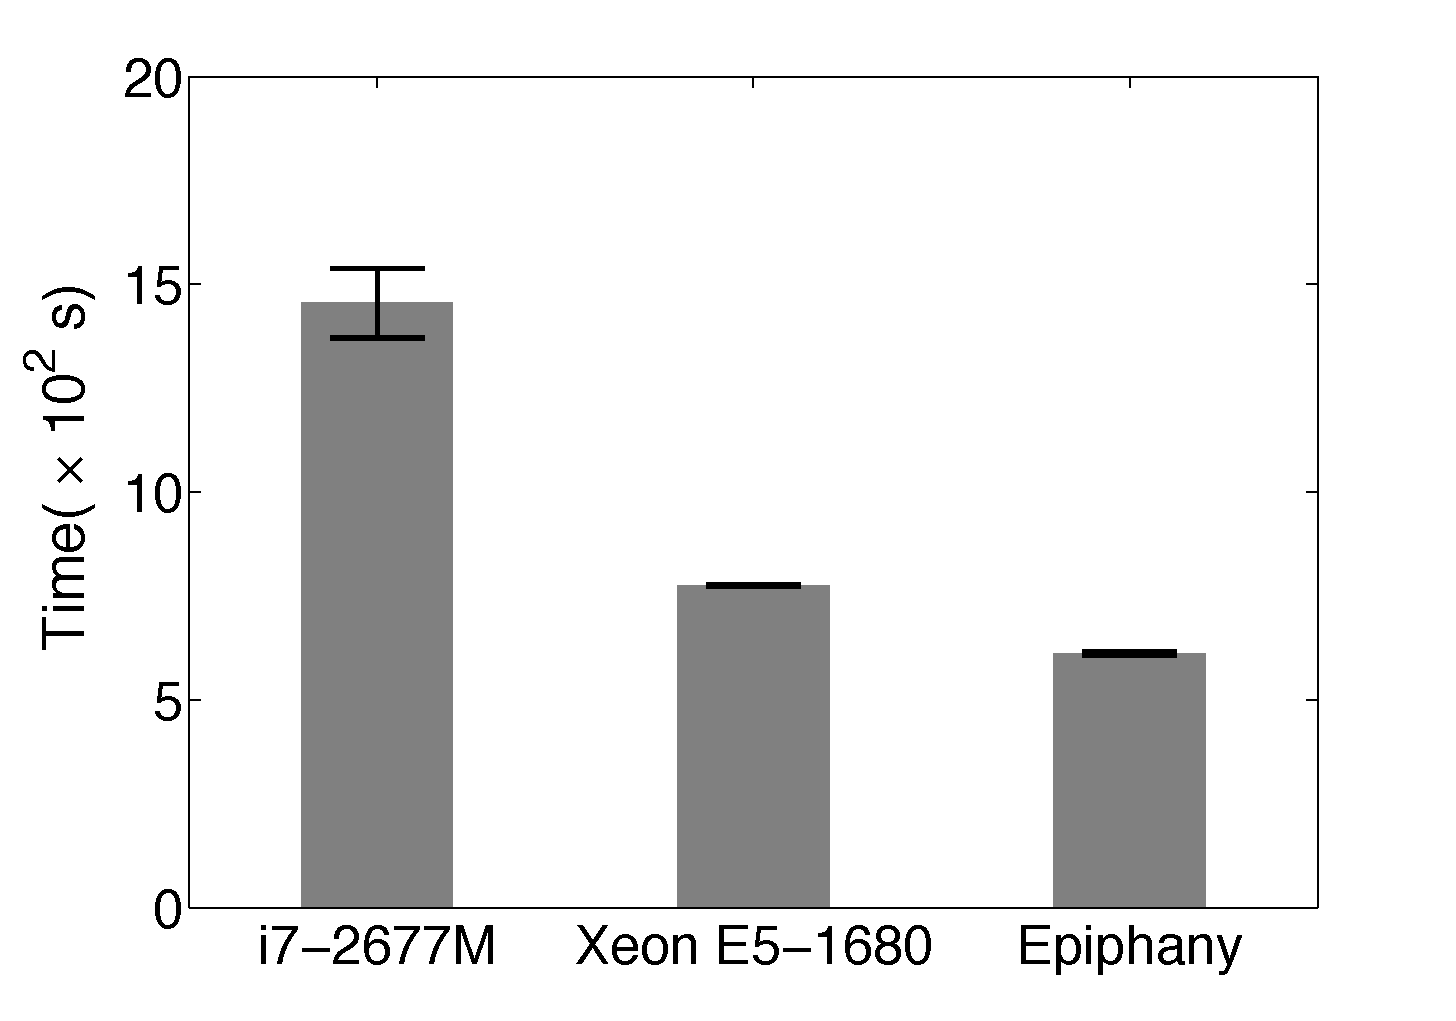
\includegraphics[width=\textwidth]{gt_5000.pdf}
	\caption{5000 records}
	\label{fig:k5000_comptime}
\end{subfigure}
\caption{Computation time for n\"{a}ive KNN search}
\label{fig:fullK256_1000_5000}
\end{figure}
Since it would have been computationally infeasible to conduct a full KNN (K=$10^6$) search over all the records in the dataset, we selected 256, 1000, and 5000 records and conducted a naive KNN search with K=256, 1000, and 5000 respectively. 
As mentioned in Section \ref{sec:methodology}, we use hamming distance as our distance. 
We ran the KNN search on a typical laptop (Macbook Air with Intel i7-2677M), high performance desktop (Mac Pro with Intel Xeon E5-1680), and on the Parallella (Epiphany III). 
Figure \ref{fig:fullK256_1000_5000} shows the comparative performance of these three processors. For 256 record dataset (Figure \ref{fig:k256_comptime}), we see that the Parallella board performs 23.05\% faster than the Macbook Air, but is slower than the Mac Pro by 13\%. 
For 1000 record dataset (Figure \ref{fig:k1000_comptime}) the board is faster than the Macbook Air by 30\%, but is slower than the Mac Pro by only 7\%. 
Finally, for 5000 record dataset (Figure \ref{fig:k5000_comptime}) we observe that the Epiphany runs 58.03\% and 21.22\% faster than the Macbook Air and Mac Pro respectively. 

\textbf{\underline{Result}}: \textit{Using the Epiphany multicore chip on the Parallella board, for a n\"{a}ive KNN search, we were able to achieve a speed up of 58.03\% and 21.22\% compared to a typical laptop and a high end desktop respectively}.

\subsection{Locality Sensitive Hashing based K Nearest Neighbour Search}
\label{subsec:lsh_knn_meas}
\begin{figure}
\centering
\includegraphics[scale=0.5]{lsh_knn.pdf}
\caption{LSH based KNN comparison}
\label{fig: lsh_knn_fig}
\end{figure}
We measured the compared the computation time of the a KNN search of 5000 records using LSH where the hash table has been constructed using the full $10^6$ record dataset on the Parallella board with a n\"{a}ive KNN search over just 5000 records on the Macbook Air and the Mac Pro with K=10. We observe from the results recorded in Figure \ref{fig: lsh_knn_fig} that the LSH based technique searching over the complete dataset on a low-power device is faster by approximately 3 and 5 times to the Mac Pro and Macbook Air devices. This result serves as a testimonial to the speed up achieved by using LSH.

\textbf{\underline{Result}}: \textit{Locality Sensitive Hashing based K Nearest Neighbour search, where the hashing table has been built over all $10^6$ records, is faster by a factor of 3 against the Mac Pro and a factor of 5 against the Macbook Air}.

\subsection{Power consumption comparison}
\label{subsec:power_cons_comp}
\begin{table}
\caption{Power Consumption in base and high states}
\centering
\begin{tabular}{| l | l |}
\hline
\textbf{Processor (Device)} & \textbf{Base power (W)}\\
\hline
Intel i7 2677M (Macbook Air) & 9.1 -- 12.0\\
\hline
Intel Xeon E5-1680 (Mac Pro) & 50.0 -- 56.3\\
\hline
Epiphany (Parallella) & 5.0 -- 5.1 \\
\hline
\end{tabular}
\label{table:power_states}
\end{table}

\begin{figure}[!ht]
\centering
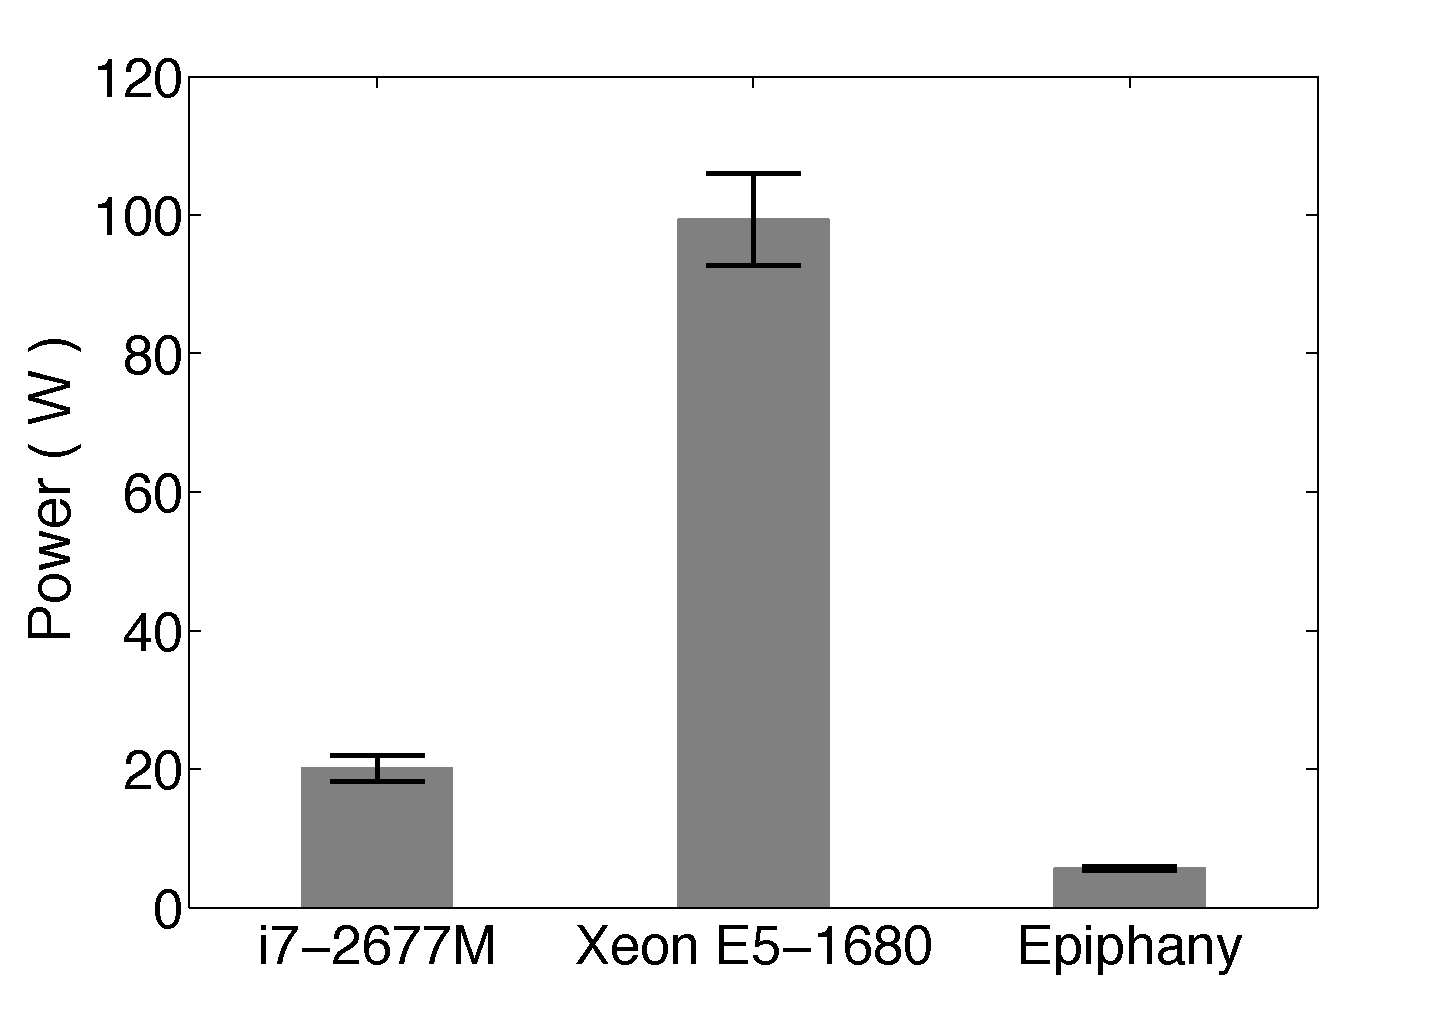
\includegraphics[scale=0.5]{powMeasure.pdf}
\caption{Power Consumption on 5000 record KNN (K =5000)}
\label{fig:pow_cons}
\end{figure}
We compared the power consumption of the Parallella board, Macbook Air, and Mac Pro for the 5000 record dataset (from Section \ref{subsec:nknn_comptime}) based n\"{a}ive KNN. The base state power consumption is shown in Table \ref{table:power_states}. Figure \ref{fig:pow_cons} shows the actual power consumed when the n\"{a}ive KNN search is being performed on the three hardware under consideration. We observe that the Epiphany processor consumes significantly less power (5.4 -- 5.9 W) than the MacBook Air (18.2 -- 22.0 W) or the Mac Pro (92.7 -- 106 W) while also computing nearest neighbours faster than either (refer to Figure \ref{fig:k5000_comptime}). 

\textbf{\underline{Result}}: \textit{The Parallella board consumes approximately 4 times less power than the Macbook Air and approximately 18 times less power than the Mac Pro for the same 5000 record based n\"{a}ive KNN (K=5000) while performing the same computations significantly faster as shown in Section \ref{subsec:nknn_comptime}}.